% Options for packages loaded elsewhere
\PassOptionsToPackage{unicode}{hyperref}
\PassOptionsToPackage{hyphens}{url}
%
\documentclass[
  9pt,
]{article}
\usepackage{amsmath,amssymb}
\usepackage{lmodern}
\usepackage{iftex}
\ifPDFTeX
  \usepackage[T1]{fontenc}
  \usepackage[utf8]{inputenc}
  \usepackage{textcomp} % provide euro and other symbols
\else % if luatex or xetex
  \usepackage{unicode-math}
  \defaultfontfeatures{Scale=MatchLowercase}
  \defaultfontfeatures[\rmfamily]{Ligatures=TeX,Scale=1}
\fi
% Use upquote if available, for straight quotes in verbatim environments
\IfFileExists{upquote.sty}{\usepackage{upquote}}{}
\IfFileExists{microtype.sty}{% use microtype if available
  \usepackage[]{microtype}
  \UseMicrotypeSet[protrusion]{basicmath} % disable protrusion for tt fonts
}{}
\makeatletter
\@ifundefined{KOMAClassName}{% if non-KOMA class
  \IfFileExists{parskip.sty}{%
    \usepackage{parskip}
  }{% else
    \setlength{\parindent}{0pt}
    \setlength{\parskip}{6pt plus 2pt minus 1pt}}
}{% if KOMA class
  \KOMAoptions{parskip=half}}
\makeatother
\usepackage{xcolor}
\IfFileExists{xurl.sty}{\usepackage{xurl}}{} % add URL line breaks if available
\IfFileExists{bookmark.sty}{\usepackage{bookmark}}{\usepackage{hyperref}}
\hypersetup{
  pdftitle={Oszilloskop},
  pdfauthor={Milena Mensching, Justus Weyers},
  pdflang={de},
  hidelinks,
  pdfcreator={LaTeX via pandoc}}
\urlstyle{same} % disable monospaced font for URLs
\usepackage[margin=1in]{geometry}
\usepackage{color}
\usepackage{fancyvrb}
\newcommand{\VerbBar}{|}
\newcommand{\VERB}{\Verb[commandchars=\\\{\}]}
\DefineVerbatimEnvironment{Highlighting}{Verbatim}{commandchars=\\\{\}}
% Add ',fontsize=\small' for more characters per line
\usepackage{framed}
\definecolor{shadecolor}{RGB}{248,248,248}
\newenvironment{Shaded}{\begin{snugshade}}{\end{snugshade}}
\newcommand{\AlertTok}[1]{\textcolor[rgb]{0.94,0.16,0.16}{#1}}
\newcommand{\AnnotationTok}[1]{\textcolor[rgb]{0.56,0.35,0.01}{\textbf{\textit{#1}}}}
\newcommand{\AttributeTok}[1]{\textcolor[rgb]{0.77,0.63,0.00}{#1}}
\newcommand{\BaseNTok}[1]{\textcolor[rgb]{0.00,0.00,0.81}{#1}}
\newcommand{\BuiltInTok}[1]{#1}
\newcommand{\CharTok}[1]{\textcolor[rgb]{0.31,0.60,0.02}{#1}}
\newcommand{\CommentTok}[1]{\textcolor[rgb]{0.56,0.35,0.01}{\textit{#1}}}
\newcommand{\CommentVarTok}[1]{\textcolor[rgb]{0.56,0.35,0.01}{\textbf{\textit{#1}}}}
\newcommand{\ConstantTok}[1]{\textcolor[rgb]{0.00,0.00,0.00}{#1}}
\newcommand{\ControlFlowTok}[1]{\textcolor[rgb]{0.13,0.29,0.53}{\textbf{#1}}}
\newcommand{\DataTypeTok}[1]{\textcolor[rgb]{0.13,0.29,0.53}{#1}}
\newcommand{\DecValTok}[1]{\textcolor[rgb]{0.00,0.00,0.81}{#1}}
\newcommand{\DocumentationTok}[1]{\textcolor[rgb]{0.56,0.35,0.01}{\textbf{\textit{#1}}}}
\newcommand{\ErrorTok}[1]{\textcolor[rgb]{0.64,0.00,0.00}{\textbf{#1}}}
\newcommand{\ExtensionTok}[1]{#1}
\newcommand{\FloatTok}[1]{\textcolor[rgb]{0.00,0.00,0.81}{#1}}
\newcommand{\FunctionTok}[1]{\textcolor[rgb]{0.00,0.00,0.00}{#1}}
\newcommand{\ImportTok}[1]{#1}
\newcommand{\InformationTok}[1]{\textcolor[rgb]{0.56,0.35,0.01}{\textbf{\textit{#1}}}}
\newcommand{\KeywordTok}[1]{\textcolor[rgb]{0.13,0.29,0.53}{\textbf{#1}}}
\newcommand{\NormalTok}[1]{#1}
\newcommand{\OperatorTok}[1]{\textcolor[rgb]{0.81,0.36,0.00}{\textbf{#1}}}
\newcommand{\OtherTok}[1]{\textcolor[rgb]{0.56,0.35,0.01}{#1}}
\newcommand{\PreprocessorTok}[1]{\textcolor[rgb]{0.56,0.35,0.01}{\textit{#1}}}
\newcommand{\RegionMarkerTok}[1]{#1}
\newcommand{\SpecialCharTok}[1]{\textcolor[rgb]{0.00,0.00,0.00}{#1}}
\newcommand{\SpecialStringTok}[1]{\textcolor[rgb]{0.31,0.60,0.02}{#1}}
\newcommand{\StringTok}[1]{\textcolor[rgb]{0.31,0.60,0.02}{#1}}
\newcommand{\VariableTok}[1]{\textcolor[rgb]{0.00,0.00,0.00}{#1}}
\newcommand{\VerbatimStringTok}[1]{\textcolor[rgb]{0.31,0.60,0.02}{#1}}
\newcommand{\WarningTok}[1]{\textcolor[rgb]{0.56,0.35,0.01}{\textbf{\textit{#1}}}}
\usepackage{graphicx}
\makeatletter
\def\maxwidth{\ifdim\Gin@nat@width>\linewidth\linewidth\else\Gin@nat@width\fi}
\def\maxheight{\ifdim\Gin@nat@height>\textheight\textheight\else\Gin@nat@height\fi}
\makeatother
% Scale images if necessary, so that they will not overflow the page
% margins by default, and it is still possible to overwrite the defaults
% using explicit options in \includegraphics[width, height, ...]{}
\setkeys{Gin}{width=\maxwidth,height=\maxheight,keepaspectratio}
% Set default figure placement to htbp
\makeatletter
\def\fps@figure{htbp}
\makeatother
\setlength{\emergencystretch}{3em} % prevent overfull lines
\providecommand{\tightlist}{%
  \setlength{\itemsep}{0pt}\setlength{\parskip}{0pt}}
\setcounter{secnumdepth}{-\maxdimen} % remove section numbering
\ifLuaTeX
\usepackage[bidi=basic]{babel}
\else
\usepackage[bidi=default]{babel}
\fi
\babelprovide[main,import]{ngerman}
% get rid of language-specific shorthands (see #6817):
\let\LanguageShortHands\languageshorthands
\def\languageshorthands#1{}
\ifLuaTeX
  \usepackage{selnolig}  % disable illegal ligatures
\fi

\title{Oszilloskop}
\author{Milena Mensching, Justus Weyers}
\date{2023-01-12}

\begin{document}
\maketitle

\hypertarget{gleichspannungsmessung}{%
\section{3.1 Gleichspannungsmessung}\label{gleichspannungsmessung}}

Das Multimeter wird in den Gleichspannungsmodus auf einen Messbereich
von \(20V\) eingestellt. Über den COM-Anschluss und den V-Anschluss wird
das Multimeter mit dem negativen und dem positiven Pol des analogen
Netzgerätes verbunden. Am Netzgerät wird daraufhin eine Spannung von ca.
\(6 V\) eingestellt. Am Voltmeter wird dann eine Spannung von \(6,06 V\)
abgelesen. Die Unsicherheit dieses Ergebnisses ist gleich der
Skalenunsicherheit des verwendeten Multimeters und beträgt:

\[u_{20V} = \frac{0,01V}{2\sqrt{3}}=0,0029V\] Damit wurde eine
Gleichspannung am Netzgerät von \(U_1 = (6,0600 \pm 0,0029)V\) gemessen.

Mittels der Bananenstecker wird das Netzgerät mit dem Kanal 1 des OZ
verbunden. Für die Auflösung in vertikaler Richtung wird eine
Kästchengröße von \(2,00 V\) eingestellt und für die Auflösung in
horizontaler Richtung eine Auflösug von \(250\mu s\), wobei diese
Auflösung bei der gemessenen Gleichspannung egal ist.

Auf dem Bildschirm des digitalen OZ erscheint daraufhin eine Linie bei 6
V. Das OZ gibt diese Spannung mit einem Wert von 6,06 Volt an. Da auch
dieses Ergebnis mit einer Genauigkeit im Hundertstelbereich angegeben
wird ist die Ungenauigkeit des Oszilloskops für diese Messung gleich
\{u\_20V\}. Damit wurde auch mit dem OZ eine Spannung von
\(U_1 = (6,0600 \pm 0,0029)V\) gemessen, die Ergebnisse sind identisch.

\hypertarget{grafische-vermessung-eines-sinusfuxf6rmigen-signals}{%
\section{3.3 Grafische Vermessung eines sinusförmigen
Signals}\label{grafische-vermessung-eines-sinusfuxf6rmigen-signals}}

Das Netzgerät und das OZ haben nach wie vor diesselben Einstellungen wie
in Abschnitt 3.2.

Mittels der zwei Cursor wird die Spitzen-Spitzenspannung an dem auf dem
Bildschirm sichtbaren Sinussignal vermessen. Das OZ gibt als
\(\Delta V\) zwischen den beiden Cursern einen Wert von
\(\Delta V = 28,0 V\) an. Dieser Wert ist mit einer Unsicherheit von
\(u_{\Delta V} = \frac{0.1V}{2\sqrt{3}}=0,029 V\) behaftet. FÜr die
Spitzen-Spitzen-Spannung ist auf graphische Weise am OZ ein Wert von
\(U_{SS}=(28,000 \pm 0,029)V\)

\hypertarget{wechselspannungsmessung}{%
\section{3.2 Wechselspannungsmessung}\label{wechselspannungsmessung}}

Das Multimeter wird in den Wechselspannungsmodus auf einen Messbereich
von 200V eingestellt. Rückblickend betrachtet wäre es besser gewesen im
Bereich von 20V zu messen. Die Unsicherheit wäre kleiner gewesen. Über
den COM-ANschluss wird das Multimeter mit dem negativen und dem
positiven Pol des analogen Netzgerätes verbunden.

\begin{figure}
\centering
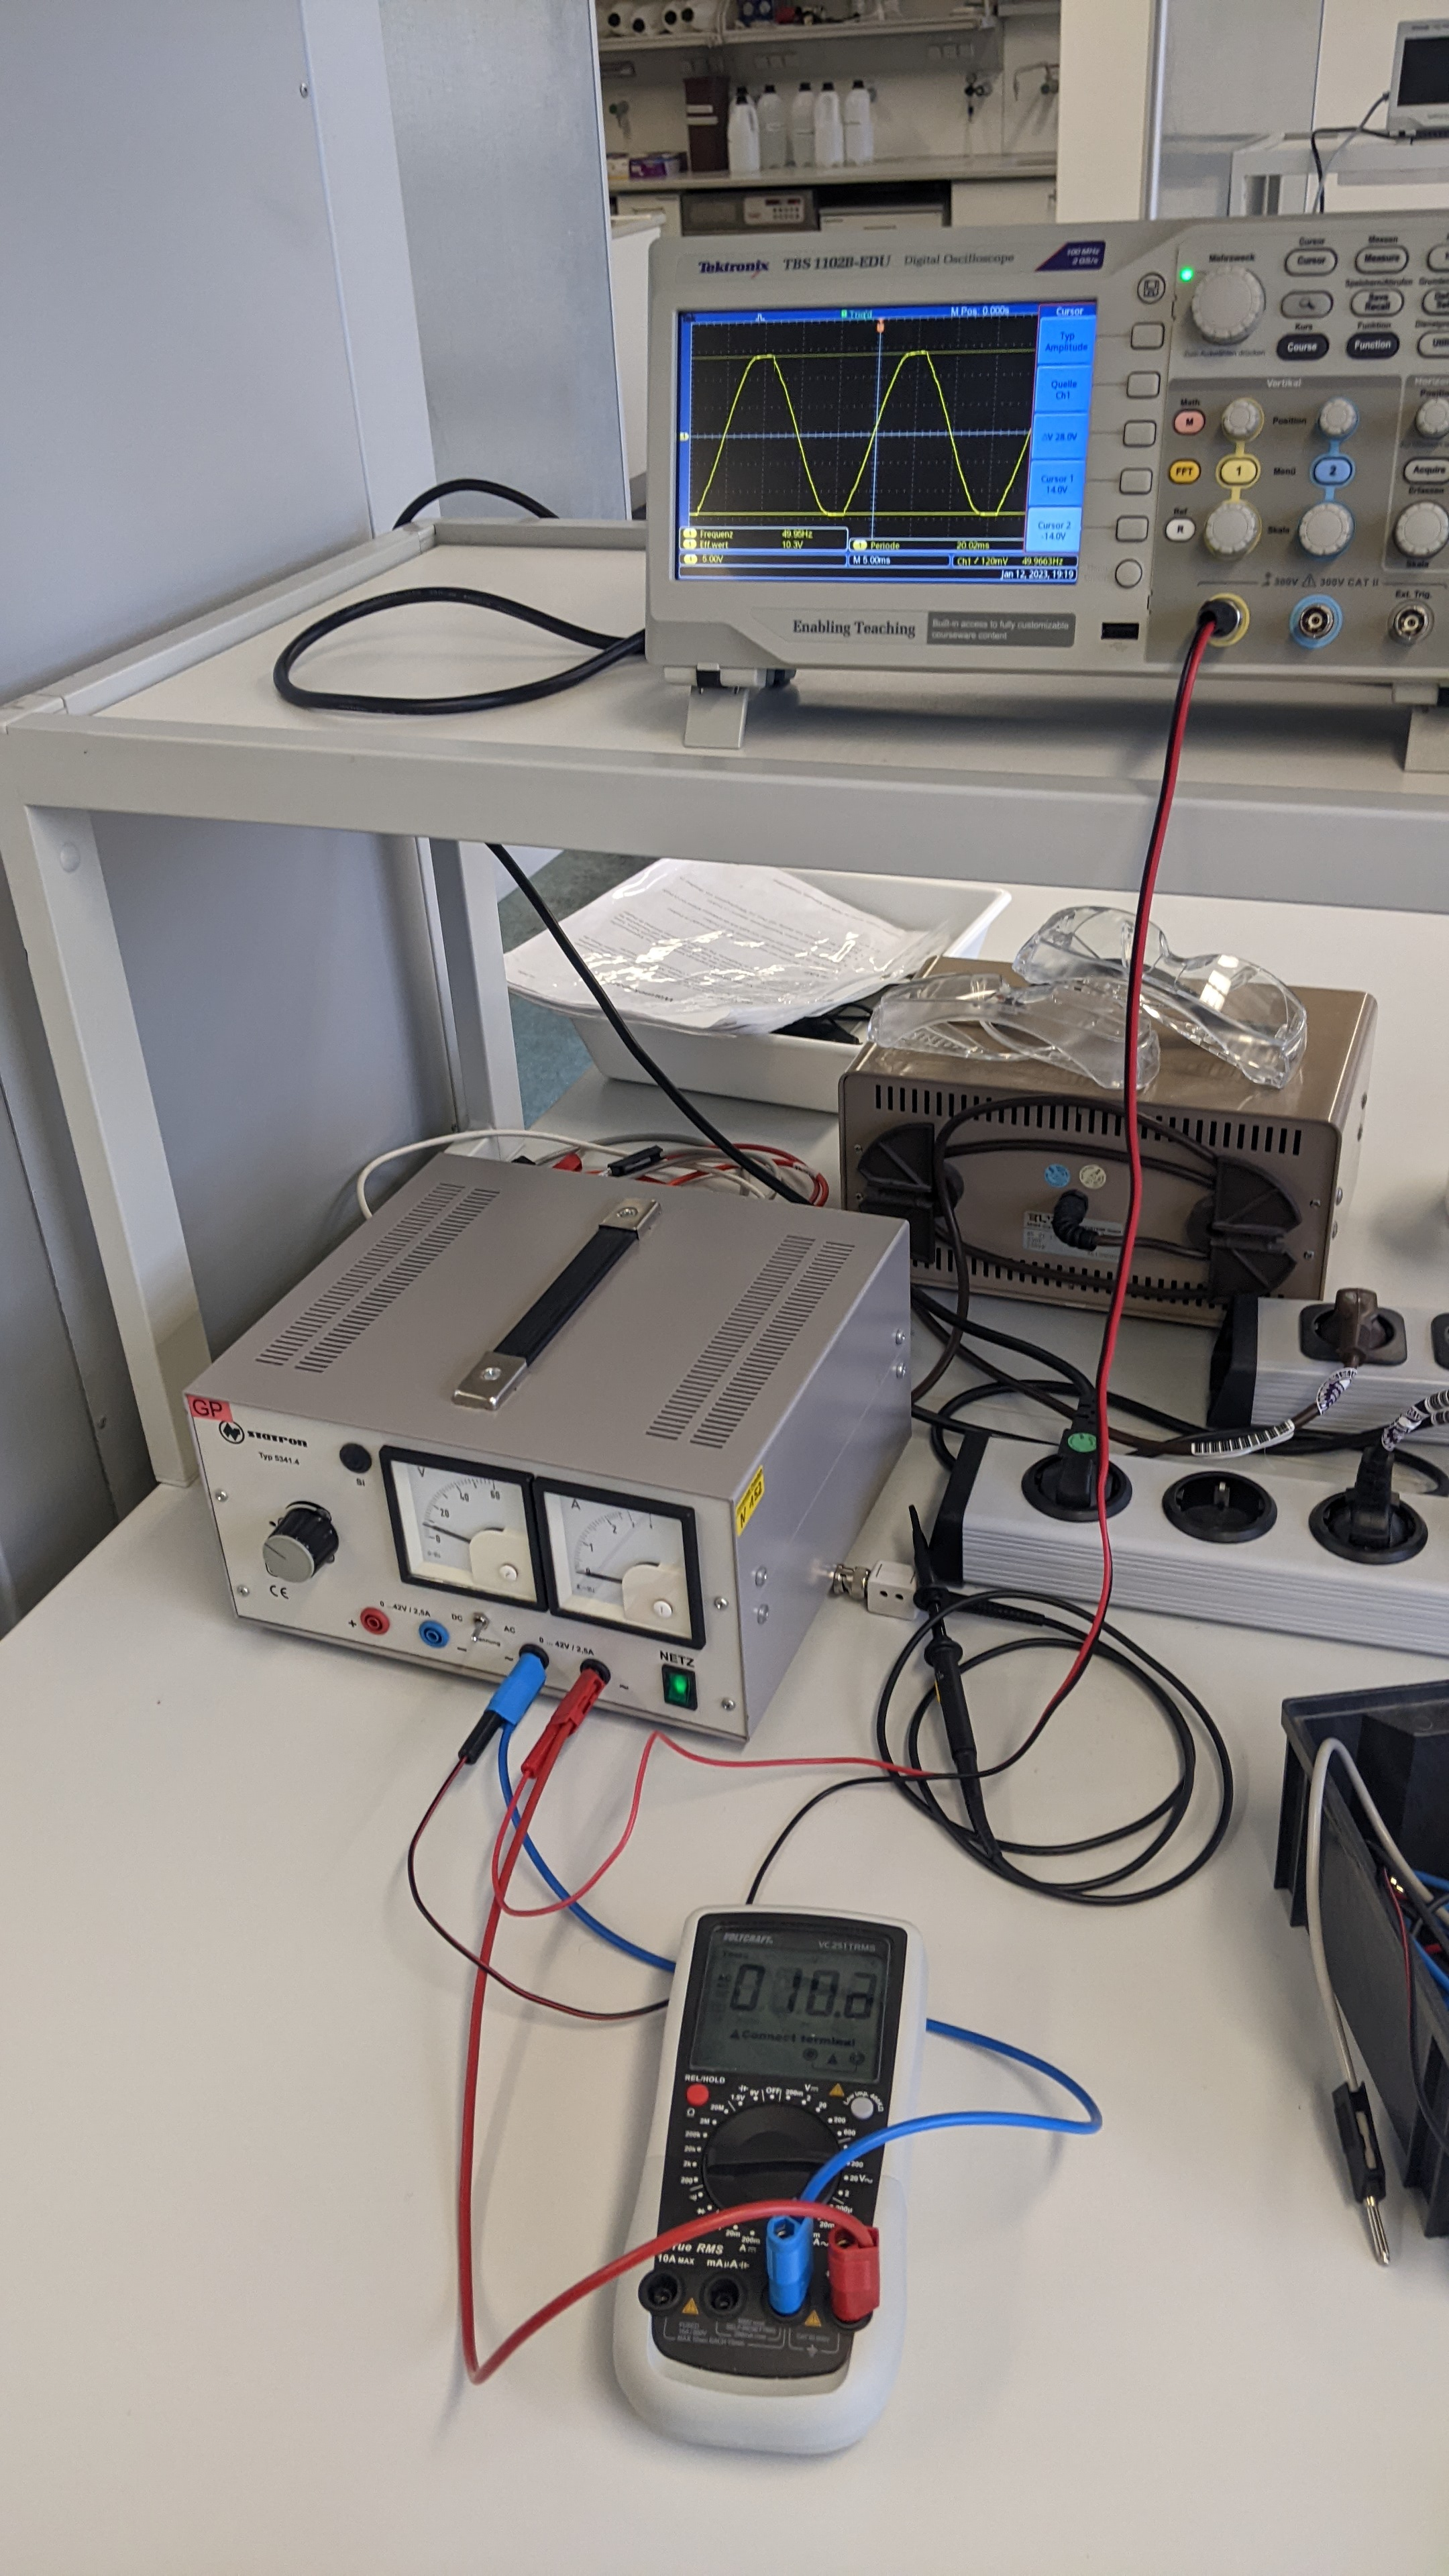
\includegraphics[width=\textwidth,height=0.2\textheight]{Bilder/3.2.jpg}
\caption{Foto von Aufbau 3.2}
\end{figure}

Die Spannung wird mit dem Multimetr auf \(U_{eff} = 10,02 V\)
(Voltmeter) eingestellt. Die Unsicherheit ergibt sich mit:

\begin{equation*}
\begin{split}
U_{Skala}&= \frac{a}{2\sqrt{3}} \\
U_{200V} &= \frac{0.1}{2\sqrt{3}} \approx 0,029V 
\end{split}
\end{equation*}

\begin{Shaded}
\begin{Highlighting}[]
\FloatTok{0.1}\SpecialCharTok{/}\NormalTok{(}\DecValTok{2}\SpecialCharTok{*}\FunctionTok{sqrt}\NormalTok{(}\DecValTok{3}\NormalTok{)) }\CommentTok{\#Unsicherheit 200V}
\end{Highlighting}
\end{Shaded}

\begin{verbatim}
## [1] 0.02886751
\end{verbatim}

Im Folgenden wurde die zuvor eingestellte Spannung von
\(U_{eff} = (10,020\pm 0,029) V\) an das Oszilloskop angeschlossen und
Spitze-Spitze Spannung \(U_{SS}\) und Periodendauer \(T\) graphisch
ermittelt. DIe Auflösung der Kästchen liegt bei \(5,00V\) in y-Richtung
und \(5,00ms\) in x-Richung. Die ermittelten Werte lagen bei
\(U_{SS} = 28V\) und \(T = 20ms\). Die Unsicherheiten ergeben sich dabei
mit:

\begin{equation*}
\begin{split}
U_{Skala} &= \frac{a}{2\sqrt{6}} \\
Spannung: U_{U_{SS}} &= \frac{1}{2\sqrt{6}} \approx 0,20V \\
Periodendauer: U_T &= \frac{1}{2\sqrt{6}} \approx 0,20ms 
\end{split}
\end{equation*}

\begin{Shaded}
\begin{Highlighting}[]
\DecValTok{1}\SpecialCharTok{/}\NormalTok{(}\DecValTok{2}\SpecialCharTok{*}\FunctionTok{sqrt}\NormalTok{(}\DecValTok{6}\NormalTok{)) }\CommentTok{\#Unsicherheit Spannung und Periodendauer}
\end{Highlighting}
\end{Shaded}

\begin{verbatim}
## [1] 0.2041241
\end{verbatim}

Insgesamt liegen die rein graphisch ermittelten Werte also bei
\(U_{eff} = (28,00 \pm 0,20) V\) und \(T = (20,02 \pm 0,20) mS\)

Mit der Periodendauer \(T = (20,00 \pm 0,20) ms\) ergibt sich eine
Frequenz von:

\begin{equation*}
\begin{split}
f &= \frac{1}{T} \\
f &= \frac{1}{20ms} = 50 Hz \\
Unsicherheit: U_f &= \frac{1}{U_T} \\
U_f &= \frac{1}{0,20ms} = 5 Hz
\end{split}
\end{equation*}

\begin{Shaded}
\begin{Highlighting}[]
\DecValTok{1}\SpecialCharTok{/}\NormalTok{(}\DecValTok{20}\SpecialCharTok{*}\DecValTok{10}\SpecialCharTok{**{-}}\DecValTok{3}\NormalTok{) }\CommentTok{\#Bestwert Frequenz}
\end{Highlighting}
\end{Shaded}

\begin{verbatim}
## [1] 50
\end{verbatim}

\begin{Shaded}
\begin{Highlighting}[]
\DecValTok{1}\SpecialCharTok{/}\FloatTok{0.2} \CommentTok{\#Unsicherheit Frequenz}
\end{Highlighting}
\end{Shaded}

\begin{verbatim}
## [1] 5
\end{verbatim}

Der Wert von \(f= (50 \pm 5) Hz\) entspricht der in Europa üblichen
Frequenz des Stromnetzes von \(50 Hz\). -\textgreater{} aber falsche
Unsicherheit

\hypertarget{digitale-messung-eines-sinusfuxf6rmigen-signals}{%
\section{3.4 Digitale Messung eines sinusförmigen
Signals}\label{digitale-messung-eines-sinusfuxf6rmigen-signals}}

Das Netzgerät und das OZ haben nach wie vor sie selben Einstellungen wie
in Abschnitt 3.2. Dieses Mal wird die Messung automatisch vom OZ durch
Drücken der Taste \(\textbf{Measure}\) ermittelt. Die beiden
ausgegebenen Werte der MEssung lagen bei \(U_{SS} = 28,2 V\) und
\(T= 20,04ms\). Die Messunsicherheit ergibt sich zu:

\begin{equation*}
\begin{split}
U_{Skala} &= \frac{a}{2\sqrt{3}} \\
Spannung: U_{U_{SS}} &= \frac{0,1}{2\sqrt{3}} \approx 0,029V \\
Periodendauer: U_T &= \frac{0,01}{2\sqrt{6}} \approx 0,0029ms 
\end{split}
\end{equation*}

\begin{Shaded}
\begin{Highlighting}[]
\FloatTok{0.1}\SpecialCharTok{/}\NormalTok{(}\DecValTok{2}\SpecialCharTok{*}\FunctionTok{sqrt}\NormalTok{(}\DecValTok{3}\NormalTok{)) }
\end{Highlighting}
\end{Shaded}

\begin{verbatim}
## [1] 0.02886751
\end{verbatim}

\begin{Shaded}
\begin{Highlighting}[]
\FloatTok{0.01}\SpecialCharTok{/}\NormalTok{(}\DecValTok{2}\SpecialCharTok{*}\FunctionTok{sqrt}\NormalTok{(}\DecValTok{3}\NormalTok{)) }
\end{Highlighting}
\end{Shaded}

\begin{verbatim}
## [1] 0.002886751
\end{verbatim}

Insgesamt liegen die digital ermittelten Werte also bei
\(U_{eff} = (28,200 \pm 0,029) V\) und \(T = (20,0400 \pm 0,0029) ms\).

Mit der Periodendauer \(T = (20,0400 \pm 0,0029) ms\) ergibt sich eine
Frequenz von:

\begin{equation*}
\begin{split}
f &= \frac{1}{T} \\
f &= \frac{1}{20,04ms} = 49,9002 Hz \\
Unsicherheit: U_f &= \frac{1}{U_T} \\
U_f &= \frac{1}{0,0029ms} = 344,83 Hz
\end{split}
\end{equation*}

\begin{Shaded}
\begin{Highlighting}[]
\DecValTok{1}\SpecialCharTok{/}\NormalTok{(}\FloatTok{20.04}\SpecialCharTok{*}\DecValTok{10}\SpecialCharTok{**{-}}\DecValTok{3}\NormalTok{) }\CommentTok{\#Bestwert Frequenz}
\end{Highlighting}
\end{Shaded}

\begin{verbatim}
## [1] 49.9002
\end{verbatim}

\begin{Shaded}
\begin{Highlighting}[]
\DecValTok{1}\SpecialCharTok{/}\FloatTok{0.0029} \CommentTok{\#Unsicherheit Frequenz}
\end{Highlighting}
\end{Shaded}

\begin{verbatim}
## [1] 344.8276
\end{verbatim}

Der Wert von \(f= (50 \pm 340) Hz\) entspricht der in Europa üblichen
Frequenz des Stromnetzes von \(50 Hz\). -\textgreater{} aber komplett
falsche Unsicherheit

\end{document}
